\documentclass[color]{tudbook}  % color: farbige Titelseite und farbige Kapitelüberschriften; nocolor: alles schwarz-weiß
\usepackage[nogerman]{tudthesis}  % german/nogerman: Sprache der Arbeit, wichtig für Titelseite, Bildunterschriften etc.
\usepackage{amsmath,amssymb}
\usepackage{setspace}   % nicht entfernen
\usepackage{graphicx}
\usepackage{subcaption}
\usepackage{hyperref}
\usepackage{mathtools}
\usepackage{enumitem}% http://ctan.org/pkg/enumitem
\DeclarePairedDelimiter\floor{\lfloor}{\rfloor}
\graphicspath{ {./images/} }


\begin{document}

% Art der Arbeit: \diplom, \beleg, \bachelor, \master
\beleg

\author{Moritz Pflügner}
\moreauthor{Matr.-Nr.: 4677226}
\title{Learned Selection Strategy for Lightweight Integer Compression Algorithm Parameterizations}
\supervisor{Prof. Dr.-Ing. habil. Dirk Habich}
\supervisorII{Dr.-Ing. Claudio Hartmann}
%optionaler Zweitbetreuer
%\supervisorIII{Betreuer 2}
\submitdate{20 October 2021}

\maketitle

\setstretch{1.2} % Anpassung Zeilenabstand an Schriftart. Bitte nicht verändern!

\newpage
% Selbständigkeitserklärung
\confirmation
\begin{abstract}
    With the continuing growth of stored data, data compression has become a common task in database systems regarding query processing or optimization. Among the large variety of existing lightweight integer compression algorithms, there is no single-best one. Thus, a selection strategy for finding suitable algorithms is necessary. In addition to the compression algorithm itself, the algorithm parameterization also influences the compression results. Hence, we present a \emph{Learned Selection Strategy for Lightweight Integer Compression Algorithm Parameterizations} which extends existing Machine Learning approaches by considering both, the selection of the best-fitting algorithm and the parameterization leading to the best compression result. We evaluate our strategy against a baseline, point out advantages of our approach and explain the behavior of our Machine Learning models by analyzing feature importances. We show that the usage of our \emph{Learned Selection Strategy for Lightweight Integer Compression Algorithm Parameterizations} lead to better compression results than using the simplest algorithm with a standard parameterization. 
\end{abstract}

\tableofcontents

\chapter{Introduction}
The amount of stored data has been increased exponentially during the last decade, reached 33 Zettabytes in 2018 and will grow to 175 Zettabytes by 2025 as the IDC \cite{Reinsel2018} predicts. This growth leads to new challenges for data processing tasks in different applications like database systems \cite{Abadi2006} or Machine Learning \cite{Elgohary2016}. Compressing the data and reducing the physical size of it has therefore become a crucial step for query executions or analytical tasks. Regarding database systems, column-organized data is usually encoded as sequence of integers \cite{Stonebraker}. Hence, the query processing is applied only to these integer sequence encoding. Compressing integer values prior to query processing leads to a better performance in terms of compression rate and ratio \cite{Woltmann2021}. Although a large variety of lightweight integer compression algorithm exists, there is no single-best one \cite{Damme2017, Damme2019} as they all behave differently regarding input data and hardware properties. Additionally, integer compression algorithms can be initialized with certain parameters like the input format, output format, or the maximum bit width of the data being compressed. The parameterization also influences the behavior of the algorithm. Selecting the best combination of compression algorithm and parameters requires a suitable selection strategy. Certain approaches have been proposed that aim to solve this task. On the one hand, rule-based strategies are based on decision trees leading to the best-fitting algorithm \cite{Abadi2006}. Cost-based approaches on the other hand define cost functions for each algorithm and choose the one with the lowest costs \cite{Damme2019}.
Strategies based on Machine Learning do not require knowledge about the algorithm behavior as it is considered as a black box. The Machine Learning model learns the behavior from training data. Regarding the algorithm selection, Machine Learning approaches lead to the best results in comparison to a cost-based and rule-based approach \cite{Woltmann2021}.
However, none of the strategies considers the best-fitting parameterization. 

In this thesis, we propose an extension of the \emph{Learned Selection Strategy for Lightweight Integer Compression Algorithms} \cite{Woltmann2021}. This extension additionally considers the best-fitting algorithm parameterization. For this, we describe the steps that are necessary in order to generate representative training data, derive features from them, create and tune the Machine Learning model, and evaluate the approach against a baseline. We show that applying a strategy which considers algorithm and parameterization leads to better compression results than using the simplest algorithm with parameters covering the largest range of data.

The thesis is structured in five chapters. Firstly, we describe general concepts of Lightweight Integer Compression, Algorithm Selection and Machine Learning in Chapter 2. Subsequently, we present the concepts and methods that will be used for the data generation process, feature engineering and hyperparameter tuning of the Machine Learning models in Chapter 3. In Chapter 4, we describe the specific implementation by presenting pipelines for the processes of data generation and validation. We evaluate the approach in Chapter 5 by using real-wold data on the one hand and by comparing it against a baseline strategy on the other hand. Finally, we conclude the thesis and give an outlook in Chapter 6. 
\chapter{Preliminaries}
The following chapter reviews and discusses related work of integer compression algorithms and adequate selection strategies in order to describe the problem the strategy presented in this thesis aims to solve. 

\section{Lightweight Integer Compression}
Lightweight integer compression algorithms is a subject of current research mainly focusing on two different objectives. On the one hand, a lot of research aims to optimize the algorithm performance with different approaches like FPGA acceleration \cite{Mohsen2020, JahanLisa2019} or novel kinds of query processing models \cite{Damme2020}. On the other hand, the research focuses on analyzing the behavior of lightweight integer compression algorithms and finding of selection strategies \cite{Abadi2006, Damme2019, Woltmann2021}.
Damme et. al \cite{Damme2017, Damme2019} have shown that among the large variety of lightweight integer compression algorithms, there is no single-best one. They all behave differently depending on the input data and hardware properties.\\
\emph{BitPacking (BP)} is one of the most frequently used algorithms in this field. One advantage that leads to good compression rates is the adaptability to different bit widths \cite{Damme2019}.\\ 
The algorithm belongs to the group of null-suppression algorithms which means that the basic idea is the omission of leading zeros in the integer binary representation. Firstly, the binary representation has to be stored as a sequence. The omission of leading zeros in every sequence element results in blocks with different sizes for every value. The size is determined by the bitwidth of the largest value in the block. 
\emph{BP} can be divided into \emph{StaticBP} where every block has a predefined size and \emph{DynamicBP} where the block size is determined dynamically.\\
Being able to analyse, compare and select lightweight integer compression algorithms in a specific context requires a non-technical abstraction. Hildebrandt et. al \cite{Hildebrandt2017} developed the COLLATE metamodel and the description language COALA for lightweight integer compression algorithms and showed that every algorithm can be modeled with it. Their work resulted in the implementation of a software framework that allows the implementation of algorithms with the COALA language, their application to input data, and the measurement of properties like compression rate or (de)compression runtime. Furthermore, the algorithms can be defined with data-dependent and data-independent parameters which change their behavior. The software framework offers the technical functionalities to observe the performance of an algorithm but for the selection of the best-fitting one, it is necessary to test all possible candidates with different parameter combinations manually and compare them according to compression rate or (de)compression runtime.

\section{Algorithm Selection}
As there is no single-best algorithm, it is necessary to determine the one that fits best for certain input data and hardware properties. In order to achieve that, an adequate selection strategy is necessary. 
In the literature, there are three major concepts. The rule-based strategy by Abadi et. al \cite{Abadi2006} is based on a decision tree for compression schemes. Certain data properties lead to specific compression algorithms. As Woltmann et. al \cite{Woltmann2021} have already analysed, an advantage of their approach is the small tree size. The effort for traversing the tree is low, but the staticness of it makes it difficult to extend it to the current landscape of algorithms.\\
Damme et. al \cite{Damme2019} developed a cost-based approach which is based on calibration measurements for each algorithm in order to retrieve the impact of data and hardware characteristics. This strategy has also been part of the analysis of Woltmann et. al \cite{Woltmann2021}. They noted on the one hand, that it can take a wide range of algorithms into account, but adding new algorithms would always require manual effort on the other hand.\\
Based on their analysis, Woltmann et. al \cite{Woltmann2021} proposed a third strategy combining the advantages of the rule-based one and the cost-based approach. Their main objective was the reduction of manual effort if a new algorithm is to be included into the selection set. Therefore, they designed their strategy as a black-box approach which does not need any information about the behavior or characteristics of the algorithm. In order to implement this, Machine Learning was used to train a model for each algorithm based on generated training data. After the training phase, the model was able to predict the cost of the algorithm when applied to certain input data.\\
As described above, lightweight integer compression algorithms behave differently due to specific input parameters. The learned selection strategy of Woltmann et. al \cite{Woltmann2021} performed better than the cost-based one by Damme et. al \cite{Damme2019}, but it can only select the best-fitting algorithm and does not take parameterizations into account.

\section{Machine Learning}
Machine Learning (ML) has become a popular technique in database systems in order to manage and analyse data. Especially tasks like data sorting \cite{Kristo2020} or cardinality estimation \cite{Kipf} are suitable for it. Considering algorithm selection, only a few ML approaches exist. Jin et. al \cite{Jin2019} proposed a selection strategy that considers the algorithm selection as a classification problem. During the training phase, they aggregate data with similar properties to data blocks and label them with the algorithm behavior. Afterwards, they predict the best-fitting algorithm by getting the data block with the lowest distance to the test data. Due to the usage of classification, adding a new algorithm would require a complete new training phase.\\
Boissier and Jenduk \cite{Boissier} developed a selection strategy based on Linear Regression and Gradient Boosting (GB) for the Hyrise database. Even though the GB model showed the best results, they left out crucial validation aspects in their work.\\
Woltmann et. al \cite{Woltmann2021} also used GB regression to train their model for the selection of the best-fitting algorithm. It is an ensemble method consisting of several weak learners, mostly decision trees. The training of every decision tree is based on the residuals of its predecessor. In comparison to the usage of Neural Networks, the times for training and forward passes are relatively low.\\
The correct interpretation of a ML model requires the evaluation of feature importances. This aspect has not been a part of the work of Woltmann et. al \cite{Woltmann2021} but would lead to a better understanding of the model decision which is crucial if a larger amount of algorithms are considered.\\
All existing ML approaches have in common that they only aim to select the best-fitting algorithm. None of them also considers the selection of algorithm parameterizations.
\chapter{Concepts and Methods}
\label{chap:concepts_and_methods}
\section{Data Generation}
In order to build a model which is able to predict the behavior of parameterized algorithms, representative training data is necessary. As in many other ML applications, this data does not exist initially which is called the cold start problem \cite{Woltmann2021}. Solving this problem requires an adequate data generator producing representative integer values which then have to be labeled with the behavior of each considered algorithm i.e the compression rate and the compression runtime. Since all lightweight integer compression algorithms need integer sequences as input data, it is necessary to derive a representation of them. A common approach is the usage of \emph{bit width histograms} (bwhist) \cite{Damme2020, Woltmann2021}. In an integer sequence, every value has a different bitwidth maximum depending on the size of the value. A bwhist of a sequence consists of \emph{b} buckets where \emph{b} is equal to the amount of bits that are used to represent the integer values of the sequence. Every bucket contains the percentual share of a specific bit width of all sequence elements.

Woltmann et. al \cite{Woltmann2021} presented multiple ways to generate representative bwhists. They showed in their evaluation that the La-Ola generator performed reasonably well even though it is the most simple strategy. The generator starts with the bwhist having a full first bucket while all other buckets are empty. 
During each iteration step a fixed percentage (percentage shift) that has been determined previously is transferred to the next bucket. The process continues until the last bucket is filled completely. The amount of bwhists being generated is determined by the amount of buckets and the percentage shift according to equation \ref{eq:amount-of-bwhist-equation} where \emph{b} is the amount of buckets, \emph{s} the percentage shift, and \emph{n} the amount of bwhists:\\
\begin{equation} \label{eq:amount-of-bwhist-equation}
    n = \floor*{\frac{1}{s}} \cdot (b-1) + 1 
\end{equation}
\begin{figure}[h]
    \centering
    \begin{subfigure}{.5\textwidth}
      \centering
      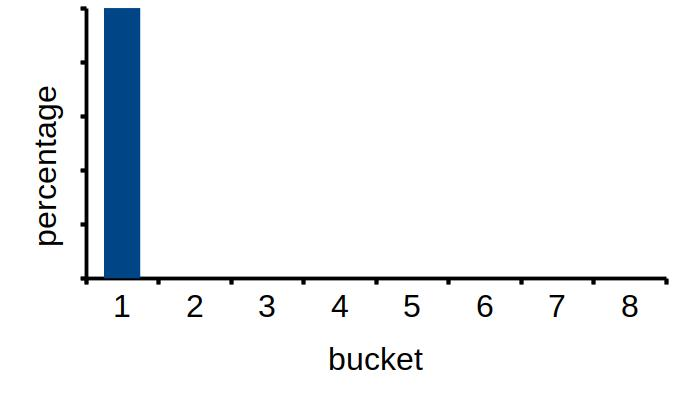
\includegraphics[scale = 0.4]{laola-1}
      \caption{bwhist 1}
    \end{subfigure}%
    \begin{subfigure}{.5\textwidth}
      \centering
      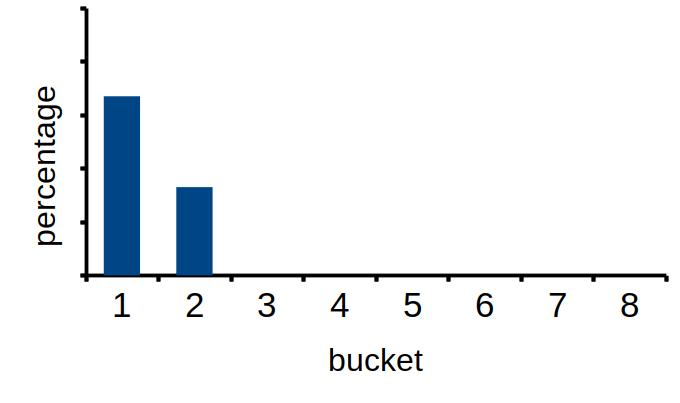
\includegraphics[scale = 0.4]{laola-2}
      \caption{bwhist 2}
    \end{subfigure}%
    \\
    \begin{subfigure}{.5\textwidth}
      \centering
      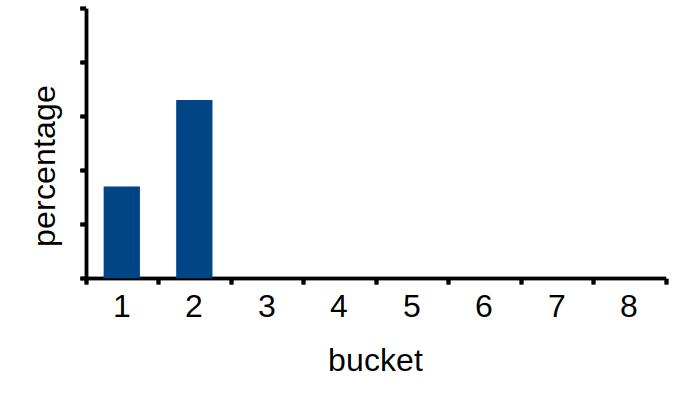
\includegraphics[scale = 0.4]{laola-3}
      \caption{bwhist 3}
    \end{subfigure}%
    \begin{subfigure}{.5\textwidth}
      \centering
      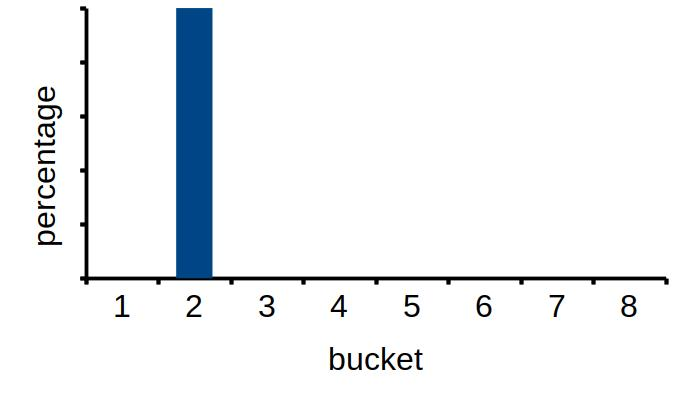
\includegraphics[scale = 0.4]{laola-4}
      \caption{bwhist 4}
    \end{subfigure}%
    \caption{La-Ola generation example for a 8-bit integer sequence and a percentage shift of 0,33.}
    \label{fig:laola-example}
\end{figure}

Figure \ref{fig:laola-example} shows the first four bwhists being generated for sequences of 8-bit integers with a percentage shift of 0,33. This La-Ola configuration would generate 22 bwhists. Due to the good ratio between simplicity and performance, we use the La-Ola approach for our data generation as well. After the bwhist generation, an integer sequence of arbitrary size can be derived.

In order to label the generated data, the implementation of the COLLATE-Metamodel \cite{Hildebrandt2017} was used as it supports multiple algorithms as well as different parameterizations. The current version of it includes \emph{StaticBP} and \emph{DynamicBP}. Therefore, only those two algorithms are considered, but the selection strategy for parameterizations can be extended for additional algorithms easily.\\
The framework supports the input format, the output format, the maximum bitwidth, and whether the sequence is sorted or not as parameters. As all of them except the output format are data-dependent, not every possible combination of parameters is valid. Therefore, only valid combinations are added to the source data before they are getting labeled.

\section{Feature Engineering}
Regarding ML, the process of feature engineering is considered as an important, but also most labor-consuming one \cite{Bengio2013}, as the quality of the model highly depends on the feature vectors it was trained with \cite{Heaton2016}.\\
After the generation of the bwhists and the integer sequences they are representing, it is necessary to derive features the ML model can be trained with. They can be divided in three classes. The first class contains features, that can be directly derived from the bwhist and have also been used for the selection strategy of Woltmann et. al \cite{Woltmann2021}. The second class contains features that have to be derived from the generated integer sequence. Class three is formed by features representing algorithm parameters.

\textbf{Class 1:}
\begin{itemize}[topsep=0pt]
    \itemsep0pt
    \item minBucket: The lowest bucket of the bwhist that contains a percentage higher than 0.
    \item maxBucket: The highest bucket of the bwhist that contains a percentage higher than 0.
    \item minPercentage: The lowest percentage of the bwhist a bucket contains. 
    \item maxPercentage: The highest percentage of the bwhist a bucket contains.
    \item averageBitwidth: The average bitwidth of the bwhist.
\end{itemize}
The average bitwidth is the weighted sum of the bitwidths the buckets are representing and its percentage.

\textbf{Class 2:}
\begin{itemize}[topsep=0pt]
    \itemsep0pt
    \item mean: The mean value of the integer sequence.
    \item stdev: The standard deviation of the integer sequence.
    \item skew: The skew of the integer sequence.
    \item kurtosis: The kurtosis of the integer sequence.
    \item isSorted: A boolean value indicating if the sequence is sorted or not.
\end{itemize}
The feature isSorted can be assigned to the following class as well, as it is also part of the algorithm parameterization.

\textbf{Class 3:}
\begin{itemize}[topsep=0pt]
    \itemsep0pt
    \item maxBitwidth: The maximum bitwidth of the integer sequence.
    \item inputFormat: The input format of every value in the integer sequence.
    \item outputFormat: The output format of every value in the integer sequence.
\end{itemize}
All classes combined lead to 13 features representing an integer sequence and algorithm parameterizations.

The COLLATE-Metamodel of Hildebrandt et. al \cite{Hildebrandt2017} supports on the one hand the measurement of the compression runtime which is the sum of the times for compression and decompression, and the compression rate on the other hand. We used both of them as target values by training one model for the compression rate and one for the compression runtime in order to compare them.

\section{Hyperparameter Tuning}
After the data generation and feature engineering process, it is necessary to train the model and tune the hyperparameters. Like Woltmann et. al \cite{Woltmann2021} we decided to use GB regression to build our ML model. In comparison to Neural Networks, the training phase of a GB model is less time-consuming. This is an important aspect for our use case as we need a ML model for every combination of algorithm and target value. Due to the consideration of the algorithms \emph{StaticBP} and \emph{DynamicBP} as well as the target values compression runtime and compression rate, four models have to be trained. Additionally, GB regression has certain hyper parameters. The number of weak learners i.e decision trees and the maximum depth per decision tree are the parameters mainly influencing the model's quality \cite{Woltmann2021}. Regarding the number of decision trees, we considered the search space \(T = [10,100] \cup{[200]}\) with a step size of 10 for the first interval. For the maximum depth per tree, the search space \(D = [3,12]\) was used.

Based on both sets, the size of the whole two-dimensional search space \emph{s} is the product of the cardinalities of \emph{T} and \emph{D} as shown in equation \ref{eq:size-of-search-space}.
\begin{equation} \label{eq:size-of-search-space}
    s = |T| \cdot |D| = 110 
\end{equation}
In order to compare the quality of the trained models, we decided to use the SMAPE metric which is the Symmetric Mean Absolute Percentage Error between a set \emph{P} of predicted values and a set \emph{A} of actual values. It is defined as follows:
\begin{equation} \label{eq:smape}
    SMAPE(A,P) = \frac{200\%}{n} \sum_{i = 1}^{n} \frac{|P_{i} - A_{i}|}{|A_{i}| + |P_{i}|}
\end{equation}
\begin{figure}[h]
    \centering
    \begin{subfigure}{.5\textwidth}
      \centering
      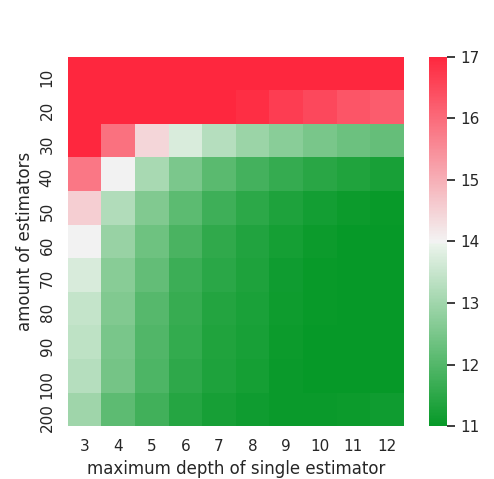
\includegraphics[scale=0.5]{ht_heatmap_dynamic_duration}
      \caption{\emph{DynBP}}
    \end{subfigure}%
    \begin{subfigure}{.5\textwidth}
      \centering
      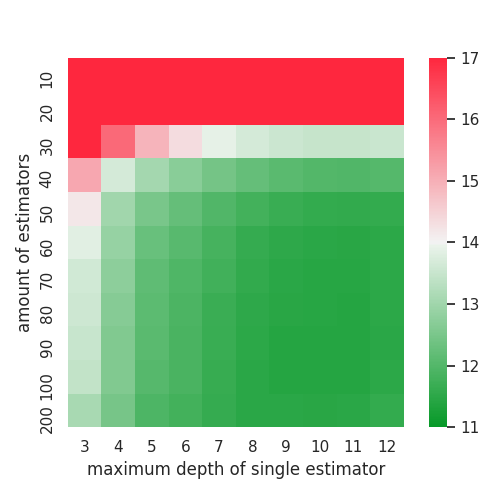
\includegraphics[scale=0.5]{ht_heatmap_static_duration}
      \caption{\emph{StatBP}}
    \end{subfigure}%
    \caption{Hyperparameter tuning results (SMAPE in \%, compression runtime as target value).}
    \label{fig:hyperparameter-heatmap-duration}
\end{figure}
\begin{figure}[h]
    \centering
    \begin{subfigure}{.5\textwidth}
      \centering
      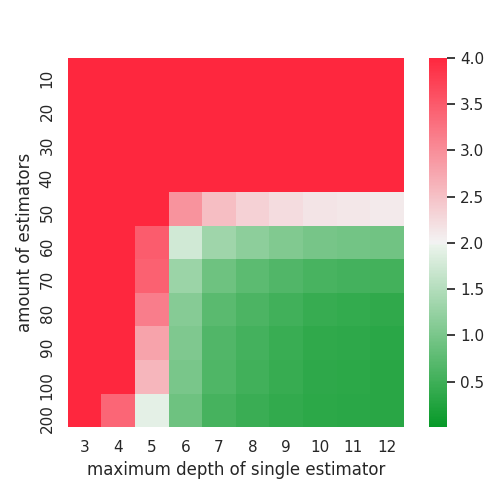
\includegraphics[scale=0.5]{ht_heatmap_dynamic_rate}
      \caption{\emph{DynBP}}
    \end{subfigure}%
    \begin{subfigure}{.5\textwidth}
      \centering
      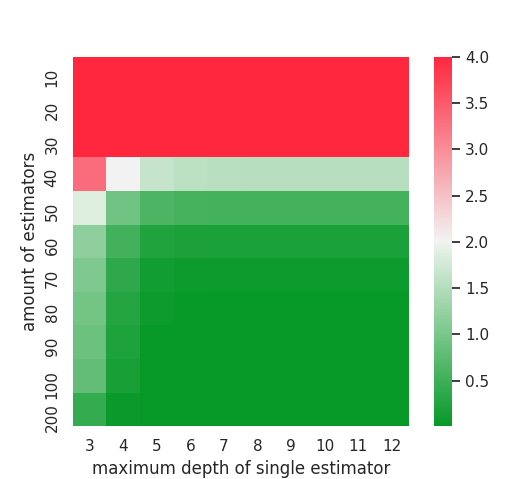
\includegraphics[scale=0.5]{ht_heatmap_static_rate}
      \caption{\emph{StatBP}}
    \end{subfigure}%
    \caption{Hyperparameter tuning results (SMAPE in \%, compression rate as target value.)}
    \label{fig:hyperparameter-heatmap-compression-rate}
\end{figure}

The hyperparameter tuning process has shown that for \emph{DynamicBP}, 80 estimators and a maximum depth per tree of 10 for both, the compression rate and the compression runtime lead to reasonably good SMAPE values while not overfitting the model.
For \emph{StaticBP},  80 estimators and a maximum depth per tree of 9 for the compression runtime and 80 estimators and a maximum depth of 6 for the compression rate lead to the best results.

\section{Conclusion}
Based on the presented methods of data generation, feature engineering, and hyperparameter tuning, a set of ML models can be trained with representative data which is the core element of the \emph{Learned Selection Strategy For Lightweight Integer Compression Algorithm Parameterizations}. Having a sequence of integers, the bwhist of it can directly be derived. Given this representation, it is possible to predict the best-fitting algorithm and its parameters by passing every possible input combination to each algorithm model and selecting the one with the best compression runtime or compression rate. 

As all of the concepts are general abstractions, a specific implementation is necessary for data generation, data labeling and model training on the one hand, as well as validation and forward passing on the other hand.  

\chapter{Implementation}
The particular implementation of the general concepts for data generation, feature engineering and hyperparameter tuning explained in Chapter \ref{chap:concepts_and_methods} can be divided into two parts. As each part consists of many single steps, we will explain our implementation with two pipeline models in this chapter. The first pipeline generates the dataset for each considered algorithm. The second one trains and tunes the ML models and validates them afterwards. Hence it depends on the output of the data generation pipeline. We split it up anyway due to the usage of two target values. The process of validation needs to be executed more often than the data generation process. 
\section{Data Generation Pipeline}
\label{ch:data_gen_pipe}
Figure \ref{fig:pipeline-data-generation} shows the pipeline for the generation of representative training data. The process is necessary as the quality of the ML model directly depends on it. The La-Ola strategy of Woltmann et. al \cite{Woltmann2021} showed the best results within their \emph{Learned Selection Strategy for Integer Compression Algorithms}. Firstly, the La-Ola Generator runs four times being configured with a percentage shift of 0.01 and multiple bucket amounts representing the input formats 8 bit, 16 bit, 32 bit, and 64 bit one after another. According to equation \ref{eq:amount-of-bwhist-equation}, it produces 11.604 bwhists in total. Afterwards, the features of the bwhist (class 1) can directly be derived.

The next step is the generation of integer values the algorithms can compress. Integer sequences passed to the algorithms of the COLLATE implementation of Hildebrandt et. al \cite{Hildebrandt2017} require a length which is integer divisable by the specified output format. Hence, an integer sequence with 800, 1600, 3200, and 6400 values is generated, representing the output formats 8, 16, 32, and 64 bit. This sampling process for combinations of input and output format increases the number of bwhists to 46.416. Furthermore, every sequence has to be considered sorted and unsorted in order to have an equal distribution of the isSorted feature. To avoid the generation of invalid data, the feature maxBitwidth is directly derived from the bwhist and not sampled. The whole process results in a list containing 92.832 samples. Completing the elements to feature vectors requires another feature extraction process deriving the features of the integer sequence (class 2) and the features representing the algorithm parameters (class 3). The feature vectors and its associated integer sequences are now exported to a CSV-File.

The next step is the labeling of every feature vector with the behavior of each algorithm i.e. the compression rate and the compression runtime. Therefore, \emph{StaticBP} and \emph{DynamicBP} are applied three times to the integer sequence of every feature vector. During the compression, the compression rates and runtimes are measured and added to the CSV-File. In order to keep the memory footprint small, the integer array is deleted after the compression process. 

The final step is the averaging of the target values of every compression process. The multiple execution and subsequent averaging ensures that the impact of outliers are flattened which results in a better ML model quality.

\begin{figure}[h]
    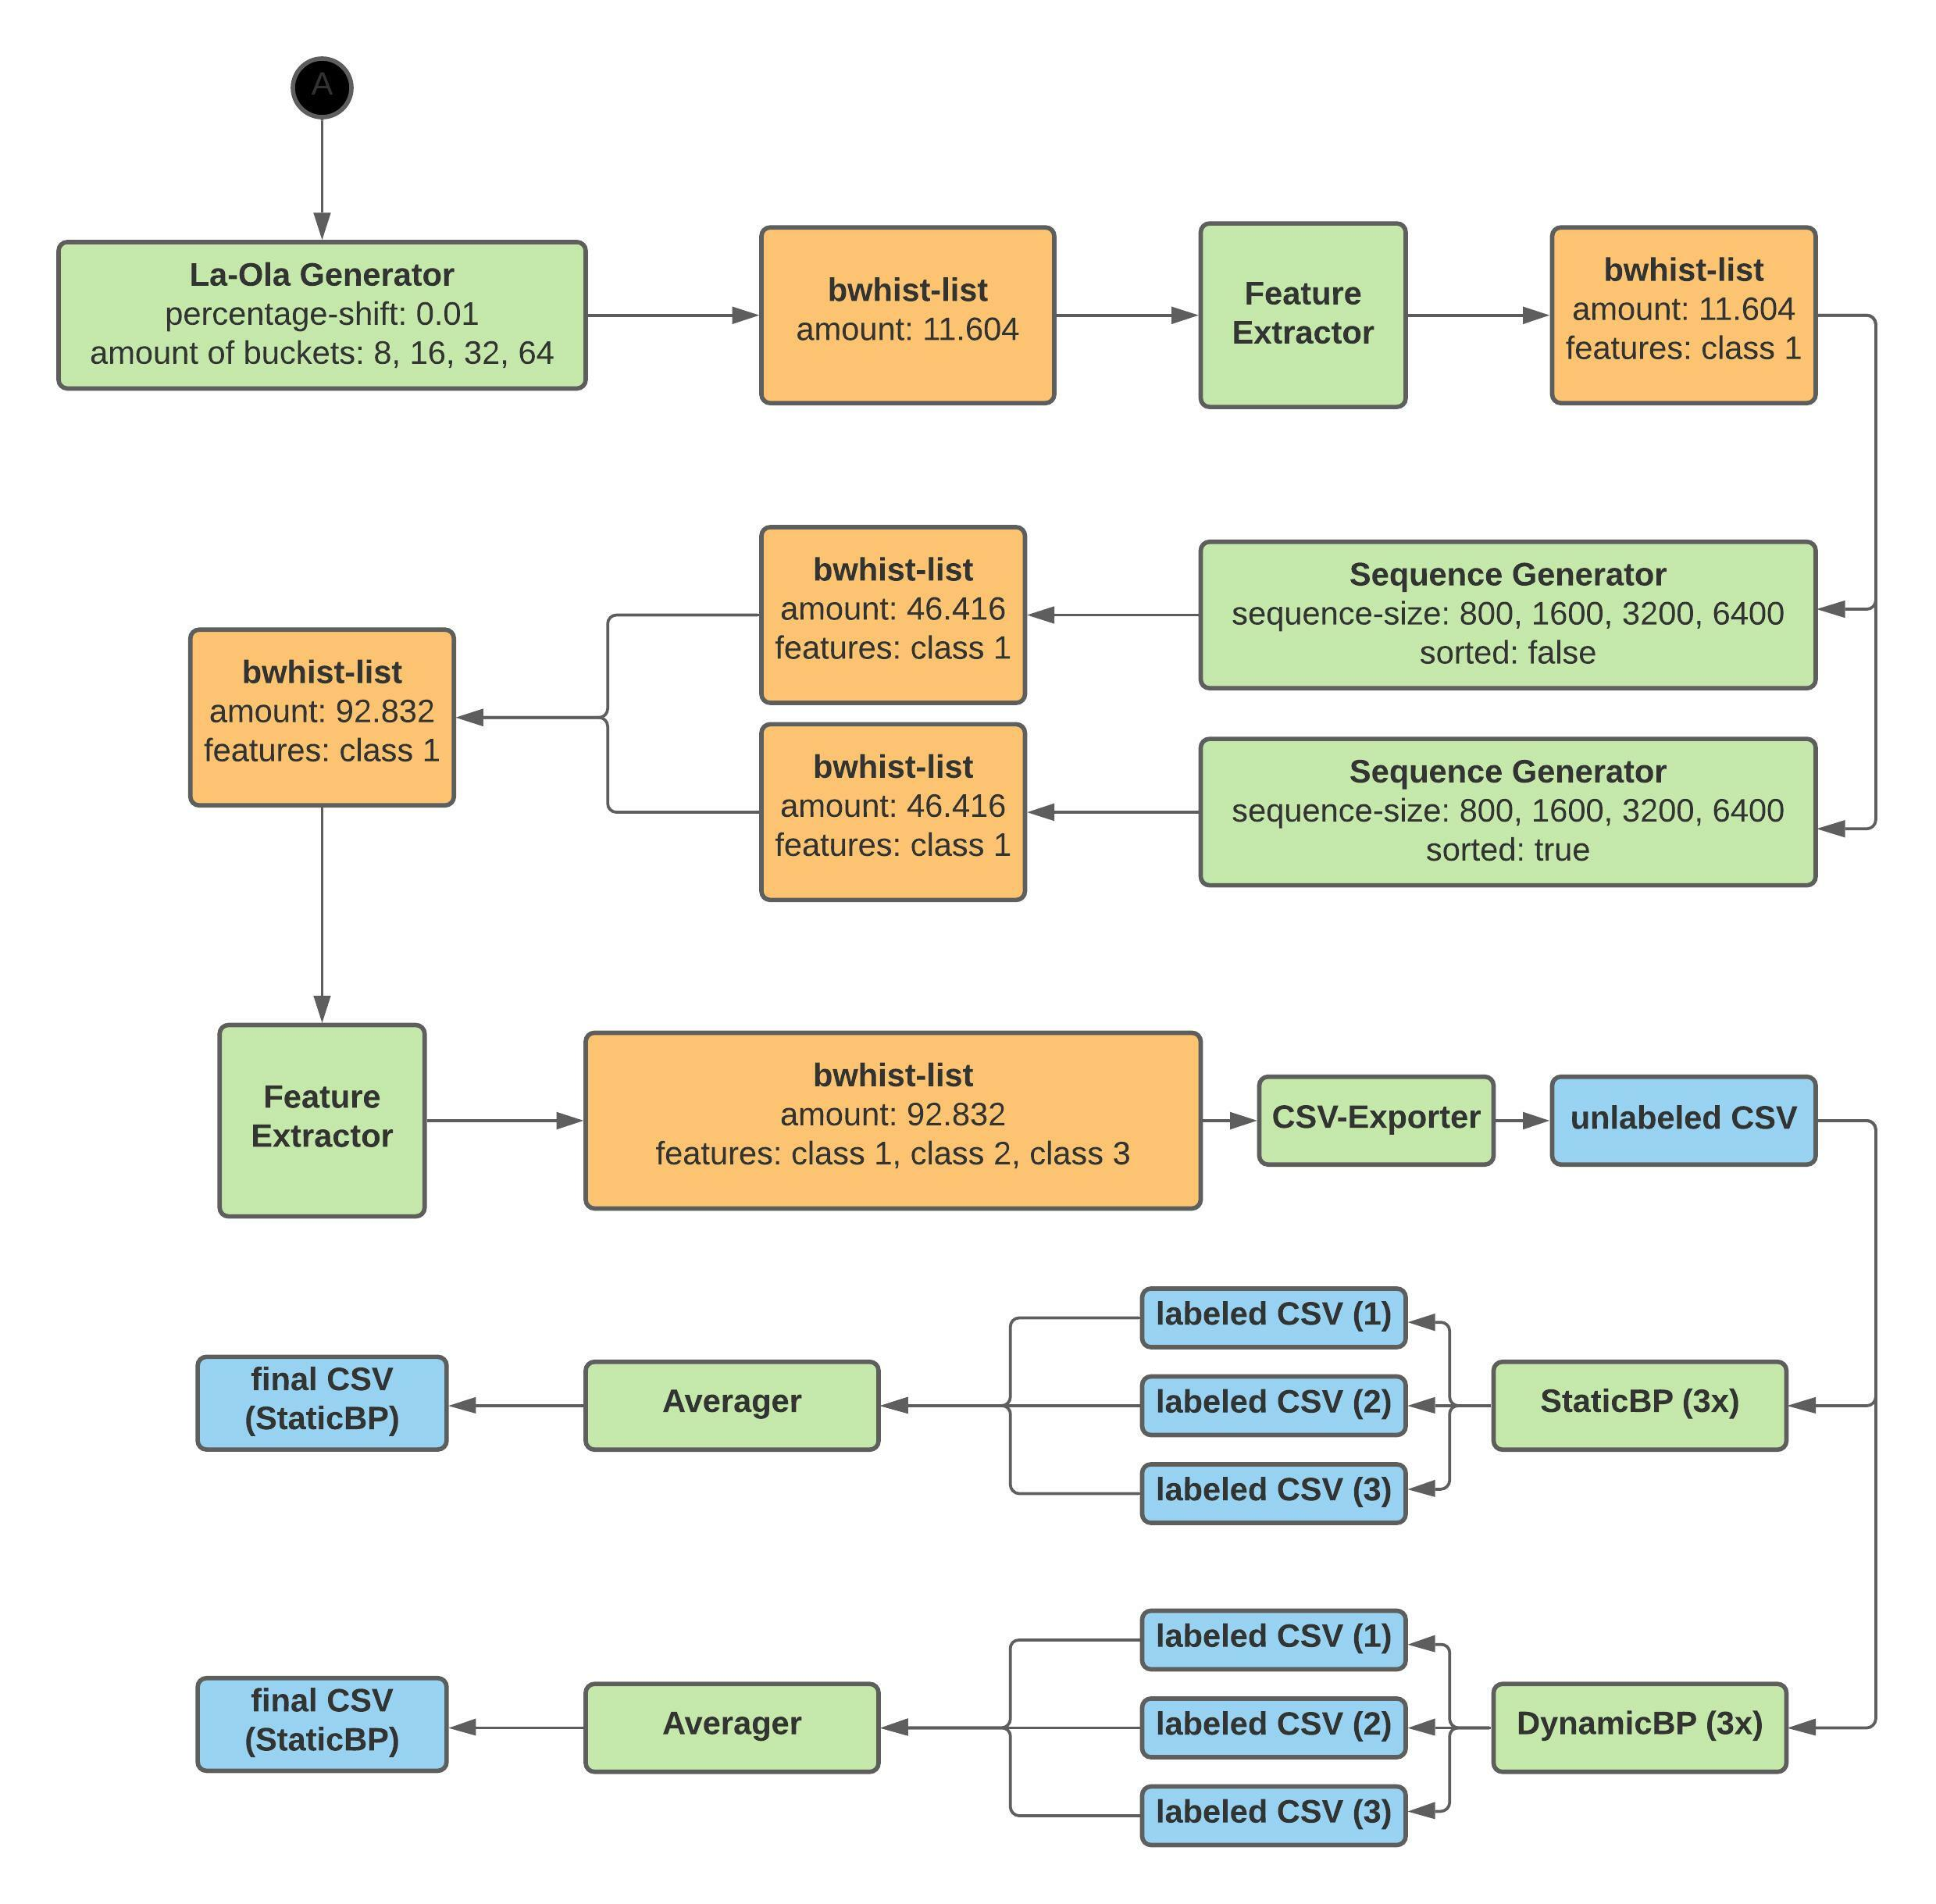
\includegraphics[width = 1.0\textwidth]{pipeline_data_generation}
    \caption{Pipeline for the generation of training data.}
    \label{fig:pipeline-data-generation}
\end{figure}

\section{Validation Pipeline}
After generating the final CSV-File containing the representative data, the ML model can be trained and tuned. The subsequent step is the validation of the ML models against the baseline selection strategy. Figure \ref{fig:pipeline-validation} shows the implementation pipeline for this process. It has to be executed once for each algorithm and for each target value. At first, a fixed subset of 20\% of the entire data set is extracted. The \emph{Algorithm Parameter Sampler} removes the features inputFormat and outputFormat as well as the target values and samples the remaining feature vector for every combination of parameters for the algorithm the data allows, for example the input format can not be smaller than the maximum bitwidth. Hence the sampling process leads to a minimum of 4 feature vectors per data sample if the maximum bitwidth is greater than 32, and a maximum of 16 feature vectors if the maximum bitwidth is smaller than 9. Figure \ref{fig:data-sample} shows an example with 16 possible combinations. 

\begin{figure}[h]
    \centering
    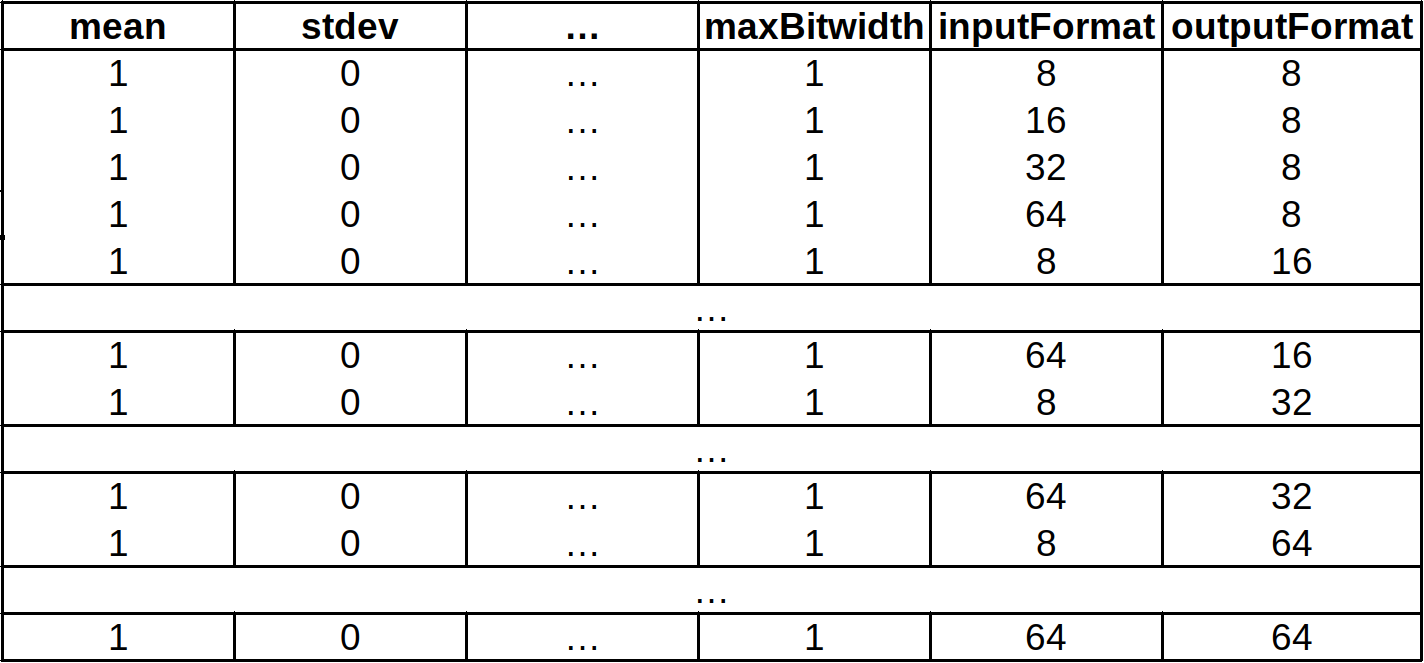
\includegraphics[width = 0.75\textwidth]{data_sample}
    \caption{Example for a feature vector sampled with 16 algorithm parameter combinations.}
    \label{fig:data-sample}
\end{figure}

The next step is the prediction of the target value. Therefore, every feature vector of the sampled test data including the parameterization of the algorithm is passed to the ML model on the one hand and to the baseline on the other hand. This leads to two datasets per algorithm and target value. The first dataset contains the target value predicted by the ML model for each feature vector. The target value of the other one represents the behavior of the baseline strategy which is the selection of the most simple algorithm i.e \emph{StaticBP} with an input format of 64 bit and an output format of 8 bit. This combination of input and output format is the most simple one as it covers all samples while having the best compression rate. 

The CSV-File generated by the data generation pipeline contains a feature vector for every possible algorithm parameter combination. In order to compare the results of the ML model and the baseline, they are passed to the \emph{Accuracy-Slowdown Processor} together with the actual data. The processor determines the minimum of the actual target values over each data sample for all algorithm parameter configuration and the minimum of both the ML model and the baseline. Now it is possible to compare, which algorithm and which parameterization would be chosen by our strategy, which one would be considered the best if the most simple algorithm is used, and which one is actually the best. Given this information, the calculation of the accuracy for the correct algorithm as well as for the correct parameterization is possible. Additionally, the slowdown can be determined, if a wrong parameterization has been chosen.

The same pipeline can be used for the validation against any data set that has been labeled with the algorithm behavior i.e compression rate or compression runtime. For this, the final CSV-File is used in order to train the ML model. This makes sure that training and test data are disjoint. The \emph{Algorithm Parameter Sampler} is then applied directly to the validation data. It is the source for the actual target values that are passed to the \emph{Accuracy-Slowdown Processor}.

\begin{figure}[h]
    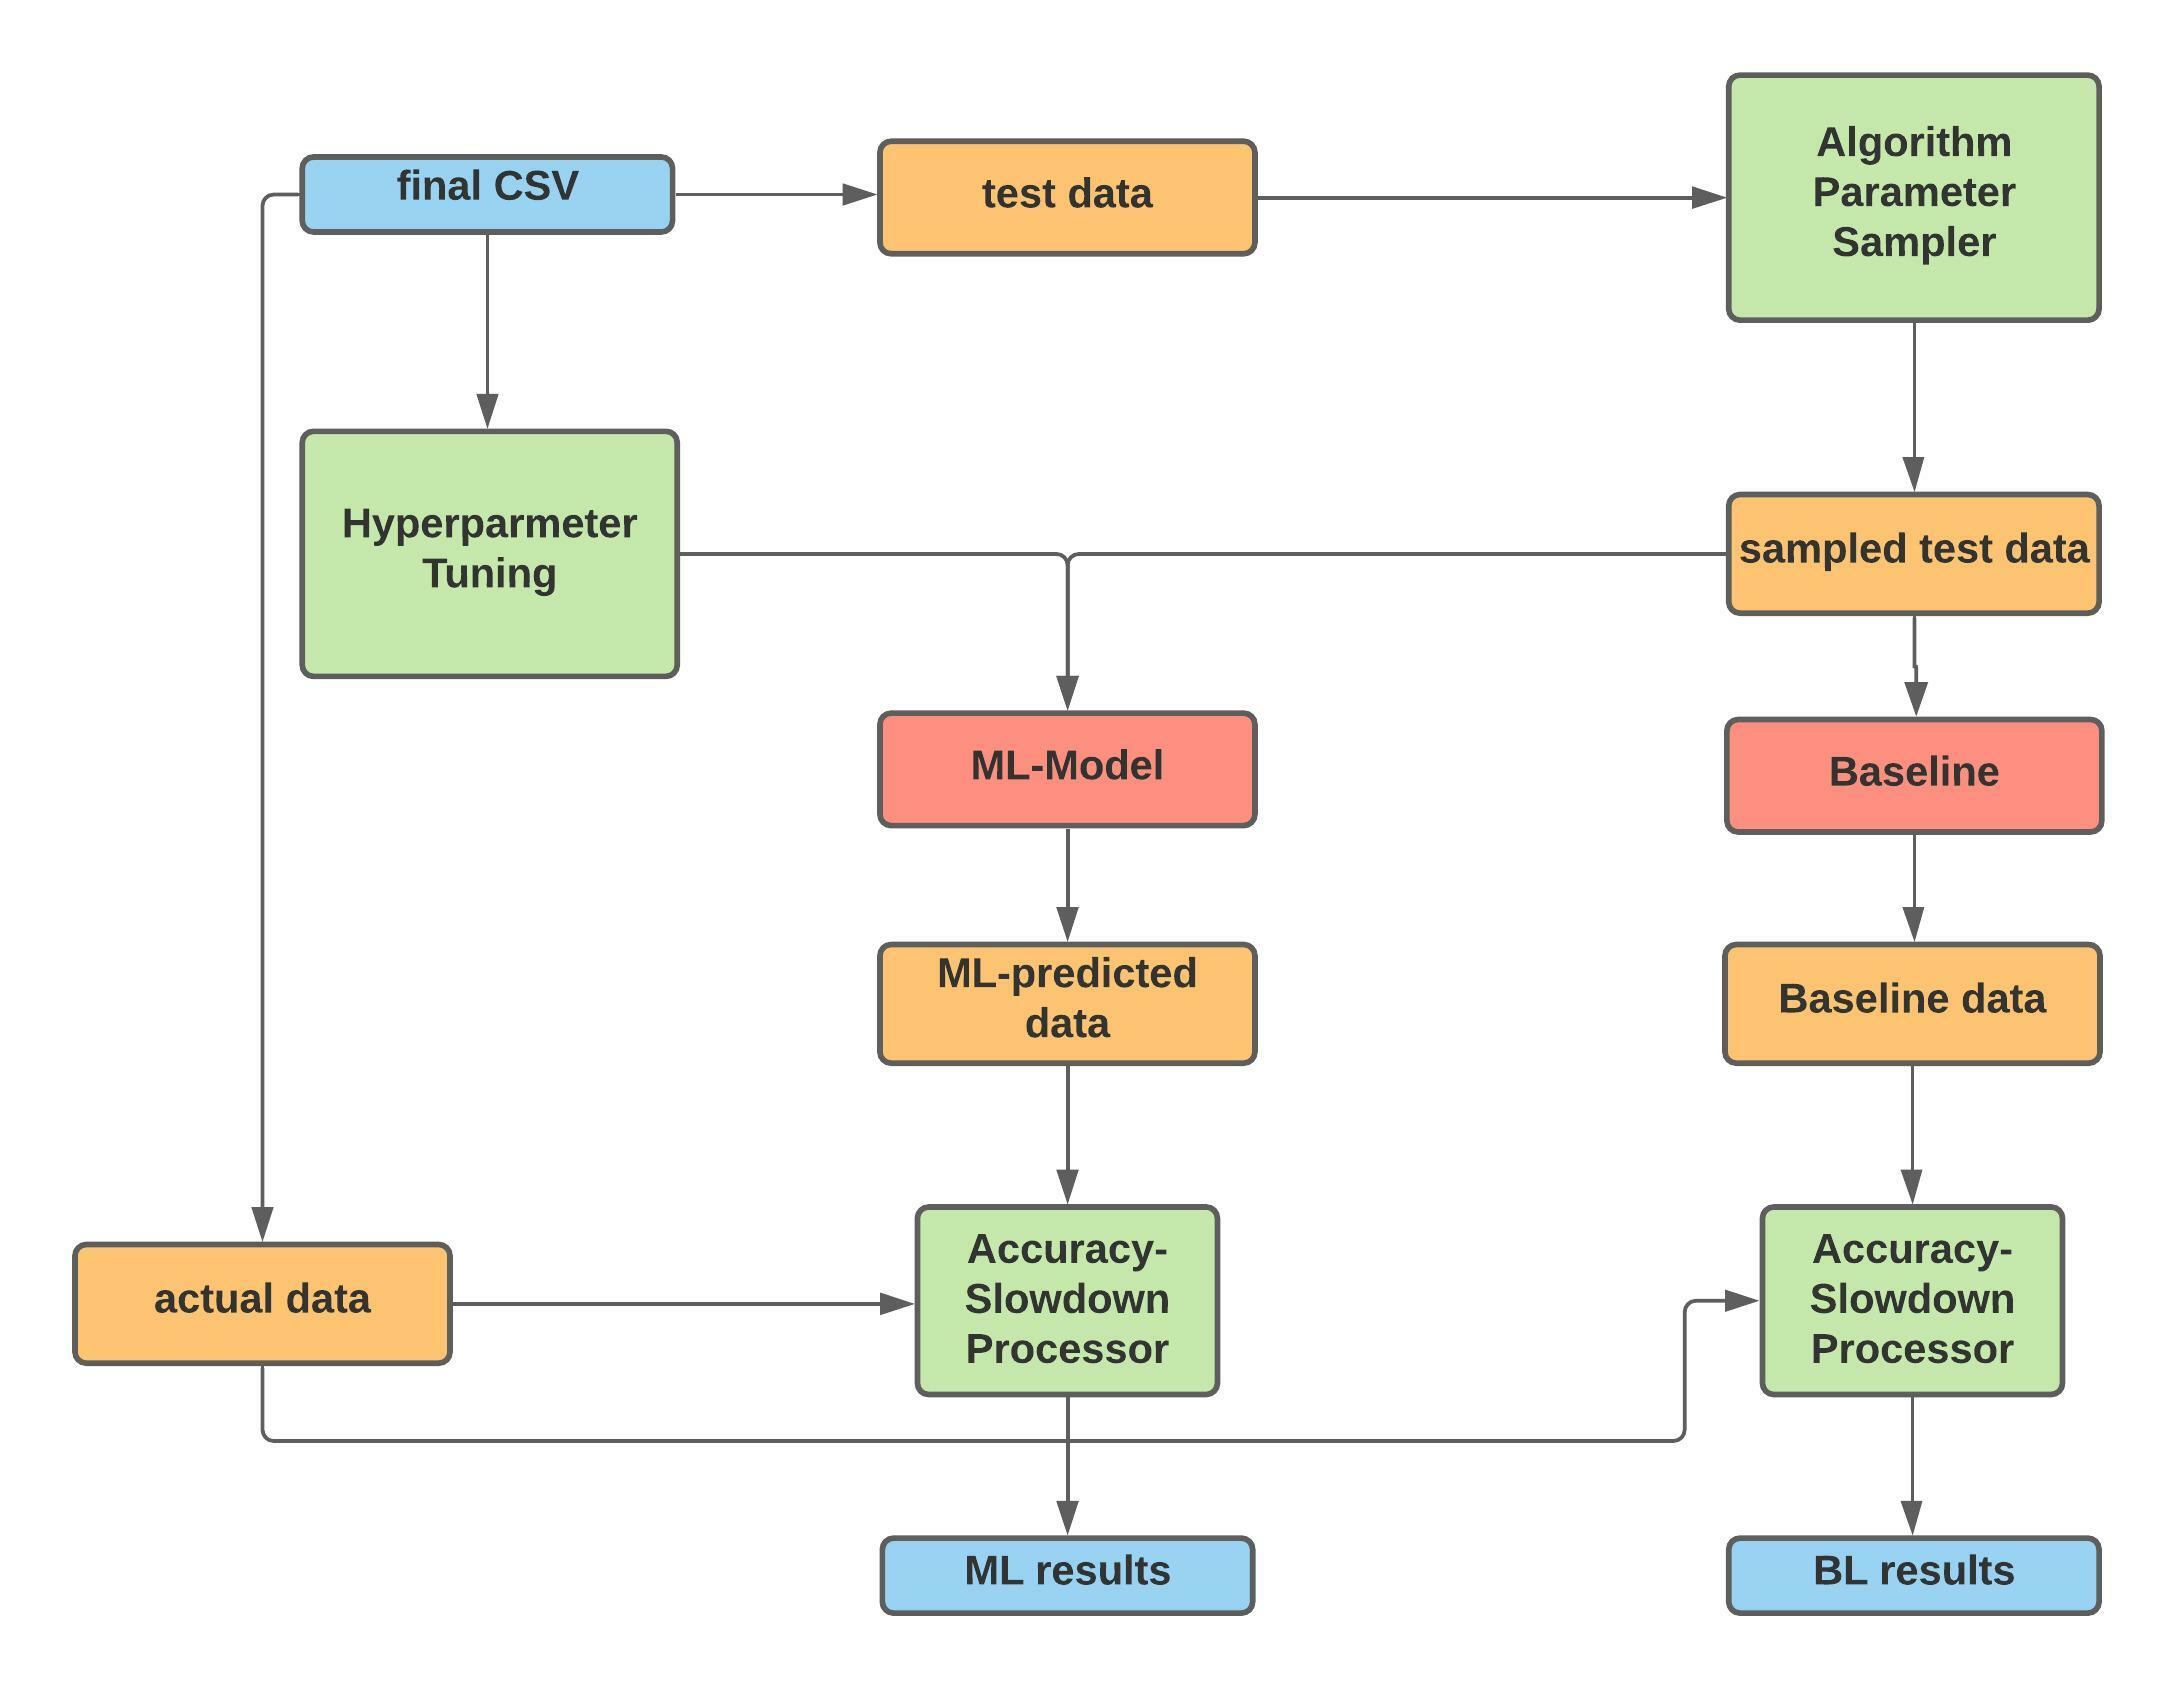
\includegraphics[width = 1.0\textwidth]{validation_pipeline}
    \caption{Pipeline for the validation process of the trained ML-Model.}
    \label{fig:pipeline-validation}
\end{figure}

\chapter{Evaluation}
This chapter contains the evaluation of our \emph{Learned Selection Strategy for Lightweight Integer Compression Algorithm Parameterizations} which is divided into three parts. Firstly, we describe our hardware setup and data sets and evaluate how long training and forward passes take. Secondly, we validate our approach against the baseline selection strategy and evaluate its performance with a validation data set. Lastly, we take a look at the feature importance in order to understand the predictions of our ML models better.
\section{Setup}
All models have been trained on a AMD Quad-Core A10-9700 APU system with 16 GB memory. The same system has been used to label the feature vectors and for application and testing of the models. The process of data labeling was necessary once by running all examples with \emph{StaticBP} and \emph{DynamicBP}. The implementation of the COLLATE metamodel by Hildebrandt et. al \cite{Hildebrandt2017} considers every different parameterization as a different algorithm and generates its implementation on the fly. This results in long compiling times before the data labeling process can start. Once labeled, the training and application of the ML model is possible.

Advantages of GB regression are the relatively fast times for training and forward passes in contrast to other methods like Neural Networks. On average, one training phase took 17.3s. Due to the fact that it was necessary to train 110 models during the hyperparameter tuning for each combination of algorithm and target value, the whole process took 127 minutes. 
For the forward passing process we measured an average duration of 390$\mu$s.

For the following validation measures, we used different data sets.
One the one hand, we used a fixed 20\% of the set generated by the La-Ola generator labeled with the compression runtime and the compression rate. This dataset is called generated data set (GDS).
On the other hand, we evaluated how our strategy performs on real-world data. Therefore we used a further data set (pBI) which consists of representative samples from the Public BI benchmark. The Public BI benchmark is a user-generated benchmark and consists of real world data represented in different tables \cite{Ghit2020}.

\section{Validation}
The ML model of our selection strategy is able to predict the optimal compression algorithm as well as the best-fitting parameters. In order to validate the quality of the predictions, we use multiple indicators. The \emph{algorithm accuracy} (aa) is the relative frequency of true positive algorithm predictions \emph{aTP} for a data set \emph{S}.   
\begin{equation} \label{eq:algo_accuracy}
    aa(aTP, S) = \frac{aTP}{|S|} \cdot 100\%
\end{equation}
Regarding the \emph{parameterization accuracy} (pa), we use the true positive predictions of the the algorithm parameters \emph{pTP}.
\begin{equation} \label{eq:param_accuracy}
    pa(pTP, S) = \frac{pTP}{|S|} \cdot 100\%
\end{equation}
Besides the calculation of the accuracy, we also consider the slowdown. It measures how much performance would be lost if the wrong prediction is chosen. As our strategy focuses on the parameterization, we decided to exclusively consider the slowdown of the wrong parameters. Having a set \emph{G} containing the target values (runtimes or compression rates) of all wrongly predicted parameterizations, a set \emph{H} containing their actual target values, and the amount of all wrongly predicted parameterizations \emph{n}, the slowdown can be calculated using the SAMPE metric.
\begin{equation} \label{eq:slowdown}
    slowdown(G,H) = \frac{200\%}{n} \sum_{i = 1}^{n} \frac{|G_{i} - H_{i}|}{|G_{i}| + |H_{i}|}
\end{equation}

In order to evaluate the quality of our ML model, a baseline is necessary. We decided to compare our model to the most simple algorithm with a parameterization allowing the compression of integer values within a range as large as possible. In particular, this baseline strategy uses \emph{StaticBP} with an input format of 64 bit and an output format of 8 bit.

The hyperparameter tuning process has shown that the hyperparameters for \emph{DynamicBP} and \emph{StaticBP} are similar. Regarding the compression rate, a more complex model is necessary for \emph{DynamicBP} in order to make predictions with the same accuracy as for \emph{StaticBP} due to the fact that the compression rate of \emph{StaticBP} can be directly derived from the parameters.

\begin{figure}[h]
    \centering
    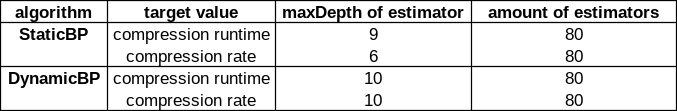
\includegraphics[scale=0.45]{hyperparameters_table}
    \caption{Result table of the hyperparameter tuning process.}
    \label{fig:table_hyperparameters}
\end{figure}

Our ML models have been trained on integer sequences with lengths of 800, 1600, 3200 and 6400 depending on the output format as described in Section \ref{ch:data_gen_pipe}. However, the input format of every integer sequence of the pBI dataset is 64 bit, but the lengths of the arrays are much bigger than the lenghts we chose for our training data. Though the sequence lengths of the pBI dataset differ for almost every sample, all of them are integer divisable by 8 what makes it possible to compress them using the COLLATE metamodel implementation by Hildebrandt et. al \cite{Hildebrandt2017}.
Due to the smaller lengths used for the training data, it is necessary to scale the predicted target value if it is proportional to the amount of integers being compressed. This is only the case for the compression runtime. The compression rate is independent of the data length. Given the output format \emph{of}, the unscaled compression runtime \emph{ur}, and the length of the integer sequence \emph{l}, we calculate the scaled runtimes (sr) for the pBI dataset according to the following equation.
\begin{equation}
    sr = \frac{ur}{of \cdot 100} \cdot {l}
\end{equation}

\begin{figure}
    \centering
    \begin{subfigure}{.5\textwidth}
      \centering
      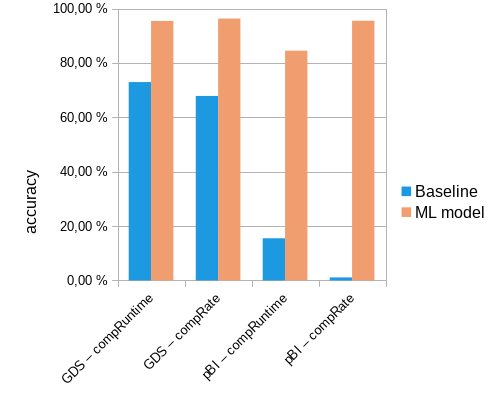
\includegraphics[scale=0.43]{accuracy_algo_new_new}
      \caption{Accuracy of algorithm selection (aa).}
    \end{subfigure}%
    \begin{subfigure}{.5\textwidth}
      \centering
      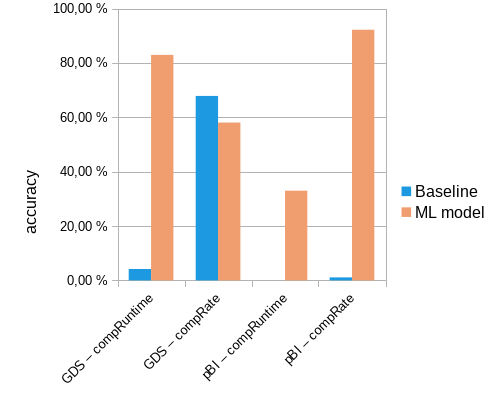
\includegraphics[scale=0.43]{accuracy_param_new_new}
      \caption{Accuracy of algorithm parameter selection (pa).}
    \end{subfigure}
    \\
    \begin{subfigure}{.5\textwidth}
      \centering
      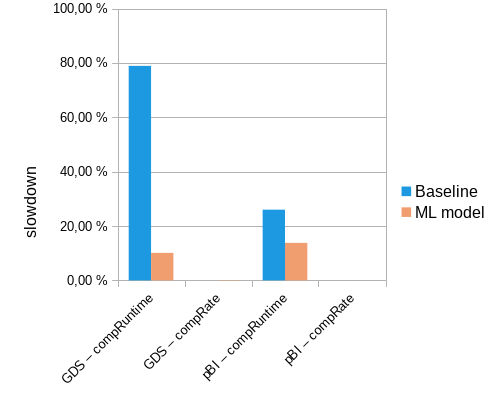
\includegraphics[scale=0.43]{slowdown_param_new_new}
      \caption{Slowdown of incorrect parameter selection (slowdown).}
    \end{subfigure}%
    \caption{Evaluation results against the generated data set (GDS) and Public BI data (pBI) considering the compression rate (compRate) and the compression runtime (compRuntime) as target values.}
    \label{fig:validation-results}
\end{figure}

The validation results presented in figure \ref{fig:validation-results} and its corresponding table \ref{fig:val_tab} show that for the compression runtime as the target value, our ML model performs better than the baseline when using our test data as well as the Public BI data regarding the algorithm selection accuracy, the algorithm parameterization selection accuracy and the slowdown. Considering the compression rate, the baseline performs better for the accuracy of the algorithm parameter selection. The baseline accuracies of 67,85\% for the test data and 1,1\% for the Public BI data are equal to the values of the algorithm selection accuracy. The reason for this lies in the way \emph{StaticBP} works. The combination of an input format of 64 bit and an output format of 8 bit always results in the best compression rate. Thus, if the baseline algorithm, i.e \emph{StaticBP} is chosen and the compression rate is used as target value, the baseline parameterization is always the best. This is also the reason for the corresponding slowdown of 0\%.

\begin{figure}[h]
    \centering
    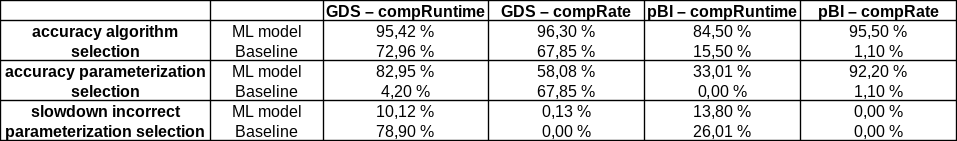
\includegraphics[width = 1\textwidth]{table_results}
    \caption{Validation table.}
    \label{fig:val_tab}
\end{figure}

The GDS is naturally more systematic and contains less outliers than the pBI dataset. Regarding the accuracy of parameterization selection, we note that our ML model performs better on the GDS when trained for the compression runtime. In contrast, it performs better on the pBI dataset when trained for the compression rate.
Due to the fact that the pBI data has different structures and properties, the model has to abstract more from the training data. Predicting the target values is therefore more difficult what results in the lower accuracies for the pBI data set than for the GDS.
Since the compression rate leads to better results for the pBI data in comparison to the compression runtime, we conclude that it is easier for the ML model to predict the compression rate than the compression runtime.
The measurement of the compression runtime is more prone to higher variations in the resulting data. The values for the compression rate on the other hand fluctuate less.

Furthermore, we observed that the ML model always reached better accuracies for the selection of the correct algorithm than for the algorithm's best parameters. The algorithm selection seems to be the easier task for the ML model than the prediction of the parameters. We expected this observation due to the different amount of possible results. While there are at worst 16 possibilities for the algorithm parameters (see Figure \ref{fig:data-sample}), there are only two for the correct algorithm.

Thus far, we evaluated our approach by considering the performance of our ML model as a whole, regardless of certain algorithm parameter combinations. In order to examine which parameter combinations lead to the best prediction results, we calculated the SMAPE for every possible combination of the input format and the output format. We do not consider the maximum bitwidth as it fully depends on the data. There are 16 different algorithm parameter combinations for the GDS. As all integer sequences of the pBI dataset have an input format of 64 bit, therefore only 4 combinations are possible. 
\newpage
\begin{figure}[h]
    \centering
    \begin{subfigure}{.5\textwidth}
      \centering
      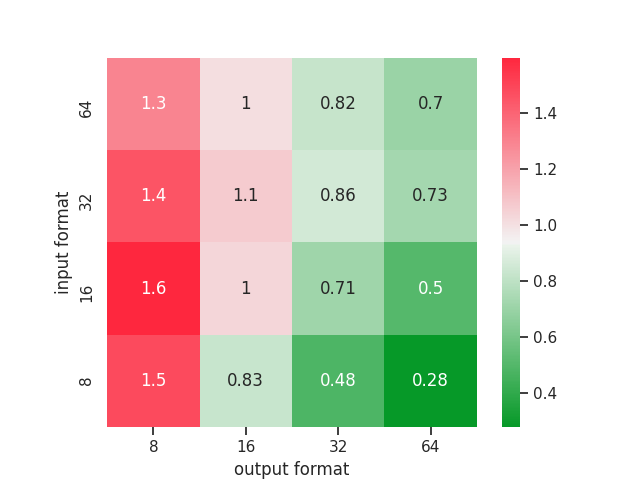
\includegraphics[scale=0.5, trim=4 0 4 4,clip]{heatmap_dynamic_compressionRate_testdata}
      \caption{compression rate}
    \end{subfigure}%
    \begin{subfigure}{.5\textwidth}
      \centering
      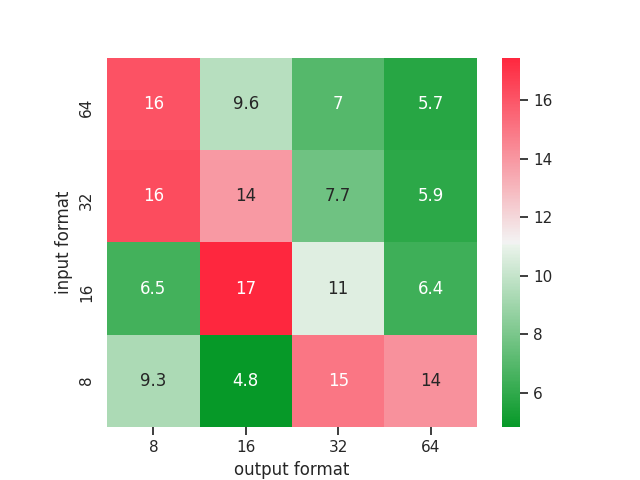
\includegraphics[scale=0.5, trim=4 0 4 4,clip]{heatmap_dynamic_duration_testdata}
      \caption{compression runtime}
    \end{subfigure}%
    \caption{Heatmap (SMAPE in \%) for single parameter combinations on the GDS for \emph{DynamicBP}.}
    \label{fig:heatmaps-single-smapes-tds-dynamic}
\end{figure}
\begin{figure}[h]
    \begin{subfigure}{.5\textwidth}
      \centering
      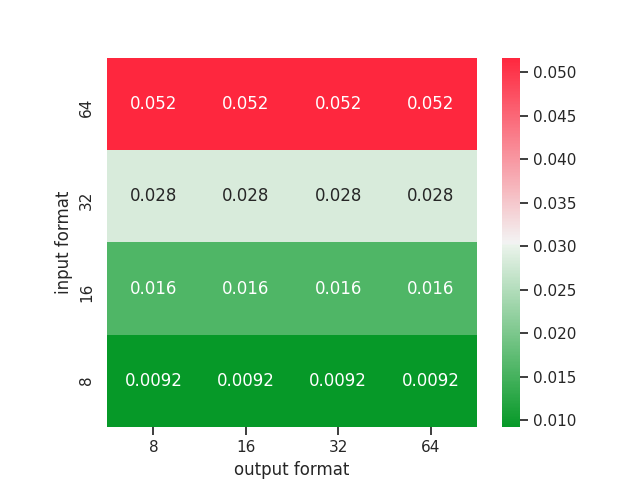
\includegraphics[scale=0.5, trim=4 0 4 4,clip]{heatmap_static_compressionRate_testdata}
      \caption{compression rate}
    \end{subfigure}%
    \begin{subfigure}{.5\textwidth}
      \centering
      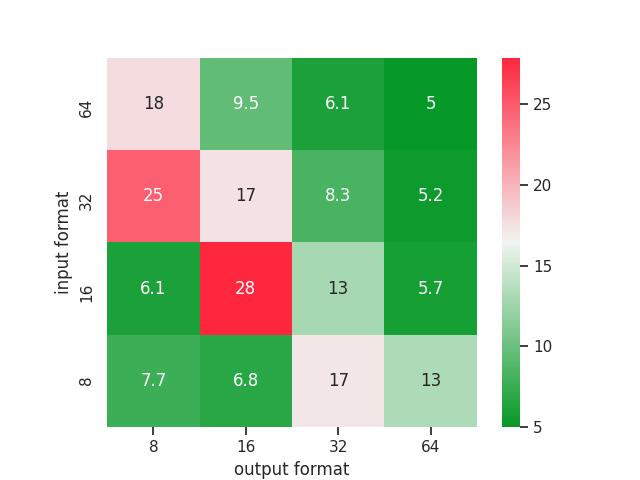
\includegraphics[scale=0.5,trim=4 0 4 4,clip]{heatmap_static_duration_testdata}
      \caption{compression runtime}
    \end{subfigure}%
    \caption{Heatmap (SMAPE in \%) for single parameter combinations on the GDS for \emph{StaticBP}.}
    \label{fig:heatmaps-single-smapes-tds-static}
\end{figure}

Figures \ref{fig:heatmaps-single-smapes-tds-dynamic} and \ref{fig:heatmaps-single-smapes-tds-static} show the SMAPE values for each possible parameter combination within the GDS. Regarding the compression runtime, the lowest SMAPE values representing better prediction results have been calculated for combinations of small input and output formats on the one hand, and for combinations of large input and output formats on the other hand. The highest SMAPE values indicating worse prediction results were determined for combinations of small input formats with large output formats and vice versa.
This behavior applies equally for both algorithms. The prediction quality of the ML model hence increases if either combinations of large input and output parameters or combinations of small input and output parameters are considered.
If a new data set is passed to the ML model in order to predict the best fitting algorithm and its parameters with the compression runtime as target value, it is useful to adjust the possible range of output format values depending on the input format(s) of the data being analysed.\\ 
In contrast to that, the prediction results of the ML model using the compression rate as target values show a different behavior for both algorithms. While the ML model performs better for \emph{DynamicBP} the larger the value for the output format, the output format has no influence on the prediction result of the ML model for \emph{StaticBP}. The reason is that the compression rate of \emph{StaticBP} is determined statically with the input format and the max bitwidth of the integer sequence.

\begin{figure}[h]
    \centering
    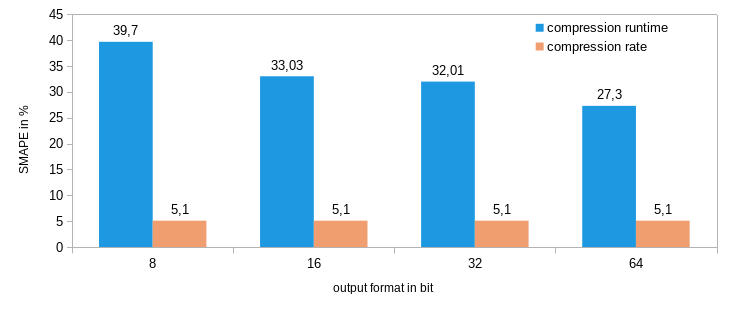
\includegraphics[width=\textwidth]{bar_chart_pbi_smapes_staticBP}
    \caption{SMAPE barchart for possible output formats (pBI dataset, \emph{StaticBP}, input format = 64 bit).}
    \label{fig:smapes_pbi_static}
\end{figure}
\begin{figure}[h]
    \centering
    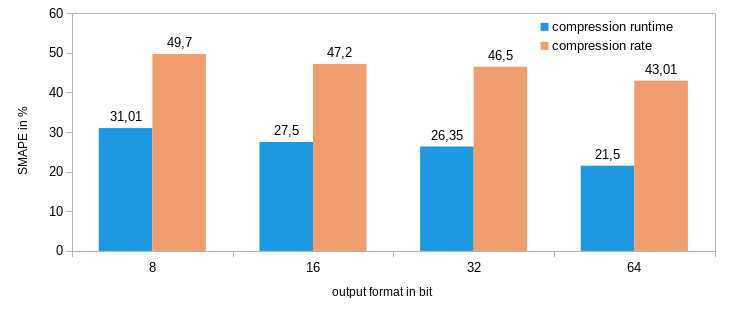
\includegraphics[width=\textwidth]{bar_chart_pbi_smapes_dynamicBP}
    \caption{SMAPE barchart for possible output formats (pBI dataset, \emph{DynamicBP}, input format = 64 bit).}
    \label{fig_smapes_pbi_dynamic}
\end{figure}

Figure \ref{fig:smapes_pbi_static} and \ref{fig_smapes_pbi_dynamic} show heatmaps containing the SMAPE values of each possible parameter combinations within the pBI data set. We can observe a similar behavior to the GDS. For every target value and algorithm, the SMAPE decreases the higher the output format is. The input format of the pBI dataset is 64 for every integer sequence. The increase in prediction quality with larger output format values fits the observation made for the GDS for an input format of 64 bit regardless the target value.   

One exception is the compression rate when using \emph{StaticBP}. Figure \ref{fig:smapes_pbi_static} shows again an equal SMAPE value for every possible output format. The reason is the same as already found for the GDS, as the functionality of the algorithms is the same for all data. 
\newpage
\section{Feature Importance}
Being able to interpret the ML models of our \emph{Learned Selection Strategy for Lightweight Integer Compression Algorithm Parameterizations} requires the consideration of feature importance. The importance of a certain feature indicates what influence it has on the model's quality. There are different ways to determine the importance of a feature. The indicator we used is the permutation feature importance \cite{Breiman2013}. 

To determine the individual importance, the following process is applied successively to every feature \cite{Breiman2013}. Firstly, the feature values get shuffled randomly over all samples which results in a decrease of the quality of the ML model. As the shuffling process breaks the relationship between the feature and the target value, the decrease is an indicator how much the target value depends on the feature. This process leads to a value indicating the decrease of the model quality and hence the importance of the feature (feature importance value).\\
We used the implementation of scikit-learn\footnote{https://scikit-learn.org/stable/modules/permutation\_importance.html, last access: 01.10.2021} which is outlined as follows:
Given the ML model \emph{m} and the training data set \emph{D}, a reference score \emph{s} is calculated indicating the quality of the model. Now, the values for each feature \emph{j} get shuffled multiple times \emph{k} which results in a corrupted version of the data set $\widetilde{D}_{j,k}$.
Now, the reference score $s_{j,k}$ is calculated for the model \emph{m} on the corrupted data set $\widetilde{D}_{j,k}$.
The importance of each feature is the difference of the reference score belonging to the original data set and the average of the corrupted reference scores.
\begin{equation}
    i_{j} = s - \frac{1}{K}\sum_{k=1}^{K} s_{k,j}
\end{equation}
\begin{figure}[h]
   \centering
   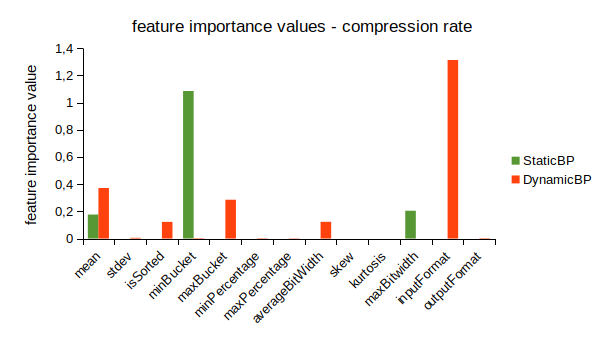
\includegraphics[scale=0.8]{feature_importance_rate}
   \caption{Feature importances for compression rate as target value.}
   \label{fig:feature_importances_compression_rate}
\end{figure}

Figure \ref{fig:feature_importances_compression_rate} shows that the ML model for \emph{StaticBP} mostly depends on the minBucket feature and the maxBitwidth feature when trained to predict the compression rate. The model for \emph{DynamicBP} mostly depends on the input format. Both observations are indicators that the ML models represent the behavior of the algorithms.
Considering \emph{StaticBP}, the block size is fixed and determined by the maxBitwidth parameter. As the minBucket feature is inversely proportional to the maxBitwidth feature, the model can derive the algorithm behavior from both features.
Regarding \emph{DynamicBP}, the bit width of a block's largest value is chosen to represent all data elements in the block \cite{Woltmann2021}. The input format correlates with the bit width of a block's largest value which is the reason for its importance.
\begin{figure}[h]
    \centering
    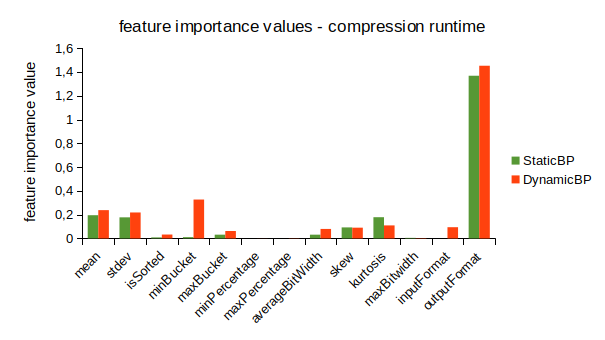
\includegraphics[scale=0.8]{feature_importance_runtime}
    \caption{Feature importances for compression runtime as target value.}
    \label{fig:feature_importances_compression_runtime}
\end{figure}

Figure \ref{fig:feature_importances_compression_runtime} shows the feature importances on the ML models when trained on the compression runtime. For both \emph{DynamicBP} and \emph{StaticBP} the outputFormat is the feature with the highest feature importance value. The output format is an indicator for the length of the integer sequence being compressed. Hence we can conclude that the longer the sequences are, the more time it takes to compress them which is an intuitive behavior. This is also the reason why it was necessary to scale the predicted compression runtime value of the pBI dataset accordingly.
Besides the output format, the features mean, stdev and minBucket have relatively high feature importance values. All three features are correlated to the size of the integer values the sequence contains. In addition to the length of the sequence, the size of the values also affects the compression runtime.

\section{Conclusion}
The evaluation of the \emph{Learned Selection Strategy for Lightweight Integer Compression Algorithm Parameterizations} has shown that its usage results in better compression results (i.e compression runtime and compression rate) than the application of the simplest approach for generated data as well as for real world data. Additionally, our learned approach results in a lower slowdown if the incorrect parameterization is chosen than the most simple approach does.
\chapter{Summary and Outlook}

Within the wide range of algorithms for lightweight integer compression, no single-best one exists \cite{Damme2017, Damme2019}. As they all behave differently depending on hardware and data properties, multiple selection strategies have been proposed \cite{Damme2019, Woltmann2021}. All of them have in common that they can determine the best-fitting algorithm but do not consider possible algorithm parameterizations. Hence, we evaluated a \emph{Learned Selection Strategy for Lightweight Integer Compression Algorithm Parameterizations} which extends the strategy of Woltmann et. al \cite{Woltmann2021}.
Firstly, it was necessary to generate representative data for training and testing with the La-Ola strategy, because our strategy is a ML based approach. From the bwhists generated by the La-Ola generator we derived 13 features representing an integer sequence. Subsequently, we applied the compression algorithms \emph{StaticBP} and \emph{DynamicBP} and labeled the data set with the compression runtime and the compression rate representing the behavior of the algorithm. For this, we used the COLLATE implementation of Hildebrandt et. al \cite{Hildebrandt2017}. With the labeled data sets, our ML models for every combination of algorithm and target value could be trained and their hyperparameters tuned. We used GB regression which requires relatively low times for training and forward passes. 
After the training phase, we evaluated the quality of our approach in comparison to a baseline strategy always choosing the most simple algorithm and the parameters that are covering the largest range of data. A test data set containing generated data and a real world data from the Public BI benchmark have been used. 
In order to increase the transparency of our ML models, we calculated the impact of each feature on the prediction result using the permutation feature importance approach.\\
We could show in our evaluation that a Learned Selection Strategy based on Machine Learning is an effective way to predict suitable parameters in addition to the best-fitting compression algorithm for certain input data. Regarding the selection results, our approach outperforms the baseline strategy in almost every case. Hence, the application of our ML based approach leads to faster or better compression results of integer values, depending on whether the compression runtime or the compression rate was used as the target value. With the analysis of the feature importance we could derive certain behaviors of our ML models. Knowing these behaviors makes it now possible to consider them during the application on new data.

We evaluated our strategy using two different integer compression algorithms. Due to the fact that our approach is an extension of the black box strategy of Woltmann et. al \cite{Woltmann2021}, no information about the algorithm behavior is necessary what makes it possible to add further algorithms without a complete new training phase. Regarding our strategy, it is firstly necessary to apply the new algorithm to our generated data. This step leads to a new labeled data set which is used to train the new ML models. In contrast to modelling the problem as classification task, our regression approach only requires a training phase for every ML model that belongs to the new algorithm. 
The new model can subsequently be used to predict the behavior of the new algorithm and hence to extend the amount of possible selection results.
Another aspect is the extension of the considered parameters. Our data generation pipeline generates all valid algorithm parameter combinations. To add a new one, it is necessary to generate a new data set based on the new possible combinations. A new data set would also lead to a new labeling process and hence to a new learning phase for every combination of algorithm and target value. A more efficient way to add new parameters would be an interesting aspect of future work. In our evaluation, we only considered the permutation feature importance. Besides, the usage of Shapley Additive Explanations (SHAP) is a common approach \cite{Lundberg2017}. While the calculation of SHAP values is more time-consuming, they can further increase the transparency of an ML model as they reveal if a feature negatively or positively influences the prediction result. Analyzing the feature importances with SHAP could also be part of future research.


\bibliographystyle{plain}
\bibliography{references}

\end{document}